\chapter{Evaluarea performanțelor obținute}
\label{chapter:eval}

Acest capitol își propune prezentarea performanțelor obținute cu ajutorul
kernelurilor pentru procesorul ConnexArray, care au fost integrate în două
blocuri de procesare din implementarea algoritmului MUSIC, și anume: blocul care
calculează un estimat al autocorelației semnalului de intrare și blocul care
calculează spectrul MUSIC. Astfel, în Secțiunea \ref{sec:eval-met} vom prezenta
modalitatea de evaluare a performanțelor și de comparare a acestora cu cea a
blocurilor din implementarea originală. Se prezintă, apoi, rezultatele obținute
pentru cele două blocuri enumerate anterior în Secțiunile \ref{sec:eval-autocorr} și,
respectiv, \ref{sec:eval-music}, respectând ordinea în care acestea apar în
lanțul de procesare MUSIC. Secțiunea \ref{sec:eval-music-chain} urmărește
rezultatele blocurilor atunci când acestea sunt integrate în întregul lanț de
procesare și, în final, în Secțiunea \ref{sec:eval-concl} stabilim concluzii și
aspecte ce ar putea fi îmbunătățite pe viitor.

%=============================================================================
% METODOLOGIE EVALUARE
%=============================================================================
\section{Metodologia de evaluare a performanțelor}
\label{sec:eval-met}

Modul de construire și execuție a lanțului de procesare, precum și utilitarele
folosite au fost detaliate în Secțiunea \ref{sec:met-eval-perf}, fiind păstrate
și în evaluarea kernelurilor ConnexArray. Compararea performanțelor
blocurilor de sine stătătoare sau a întregului lanț de procesare se va face
operând pe același set de date de intrare citite dintr-un fișier și comparând
timpul în care acestea finalizează procesarea. \\

Este important de notat faptul că ne interesează timpul petrecut în execuția
programului, în termenii percepției umane, denumit și \textit{wall-clock time}
sau \textit{wall-time}, și nu timpul petrecut pe procesor (\textit{CPU time}).
Timpul petrecut pe procesor se referă la durata care a fost petrecută procesând
date efectiv pe procesor, fără a lua în considerare și timpul de așteptare după
datele de intrare sau cel necesar pentru sincronizarea între mai multe fire de
execuție. Având în vedere că GNU Radio poate lansa mai multe fire de execuție
pentru procesare, care pot avea anumite dependențe de sincronizare, este posibil
ca timpul petrecut pe procesor să nu reflecte realitatea cu acuratețe, motiv
pentru care vom compara timpul total de execuție a programelor. \\

Putem măsura timpul total de execuție cu metoda prezentată în Anexa
\ref{sec:measure-time} (valabilă doar pentru standardul C++11), cu o precizie de
ordinul milisecundelor, care este suficientă pentru datele folosite în cazul de
față. Deoarece acesta poate să difere de la o execuție la alta din diverse
motive, precum imprecizia metodei care măsoară timpul sau evenimente hardware
care pot modifica timpul de acces la date, pentru fiecare caz analizat s-a
efectuat un număr de 10 măsurători și s-a făcut o medie a timpului obținut. \\

Toate rezultatele au fost obținute pe placa de dezvoltare Xilinx ZedBoard
Zynq-7000, pe al cărei chip FPGA se află implementat acceleratorul ConnexArray,
cu o dimensiune a liniilor de procesare de \SI{256}{B}, care include 128
elemente de procesare și o memorie locală de \SI{256}{KB}.

%\todo{Profil de putere?}

%=============================================================================
% EVAL BLOC AUTOCORELATIE
%=============================================================================
\section{Evaluarea performanțelor blocului ce calculează autocorelația
semnalului de intrare}
\label{sec:eval-autocorr}

\subsection{Procesare liniară}

În forma sa descrisă în Secțiunea \ref{ssec:gnuradio-kernel-autocorr}, blocul de
autocorelație nu realizează decât o mică paralelizare în prelucrarea datelor de
ieșire din accelerator, comportarea sa fiind, în mare parte, liniară. Realizăm
un profil conform metodologiei descrise în secțiunea anterioară pentru un sistem
cu următoarea configurație:
\begin{itemize}
  \item Număr antene: 4
  \item Număr semnale de intrare: 2
  \item Dimensiunea spectrului MUSIC: 1024
  \item Dimensiunea capturii pentru autocorelație: 2048
  \item Intervalul de suprapunere dintre capturi: 512
\end{itemize}

%=============================================================================
% Profiling table
%=============================================================================
\begin{table}[H]
\begin{center}
 \begin{tabular*}{\textwidth}{||c @{\extracolsep{\fill}} c @{\extracolsep{\fill}} c @{\extracolsep{\fill}}||}
% {||c c c||} 
 \hline
 Overhead  & Command & Symbol \\ [0.5ex] 
 \hline\hline
 43,67\% 
 &
 autocorrelate\_cnx\_impl
 &
 \makecell{gr::doa::autocorrelate\_cnx \\ \_impl::prepareInData}
 \\ 
 
 \hline
 9,75\%
 &
 autocorrelate\_cnx\_impl
 &
 \makecell{std::complex<float>::imag[abi:cxx11]}
 \\
 
 \hline
 9,53\%  
 &
 autocorrelate\_cnx\_impl
 &
 \makecell{std::complex<float>::real[abi:cxx11]}
 \\
 
 \hline
 1,89\%  
 &
 autocorrelate\_cnx\_impl
 &
 \makecell{\_\_copy\_from\_user}
 \\
 
 \hline
 1,86\%  
 &
 autocorrelate\_cnx\_impl
 &
 \makecell{\_\_gnu\_cxx::new\_allocator \\ <unsigned short>::~new\_allocator}
 \\
 
 \hline
 1,64\%  
 &
 autocorrelate\_cnx\_impl
 &
 \makecell{\_raw\_spin\_unlock\_irqrestore}
 \\ [1ex] 
 \hline
\end{tabular*}
\end{center}
\caption{Profil pentru blocul de autocorelație care folosește un kernel ConnexArray}
\label{tab:prof-autocorr-kernel}
\end{table}


Rezultatele obținute au fost sintetizate în Tabelul
\ref{tab:prof-autocorr-kernel}.  Un profil realizat asupra blocului original de
autocorelație din Tabelul \ref{tab:prof-autocorr} pe același set de date cu
aceeași configurație ne indică faptul că am reușit să eliminăm o mare parte din
punctele critice implicate în înmulțirea de matrice, cu prețul unui
\textit{overhead} semnificativ introdus de pregătirea datelor de intrare, care
consumă 43,67\% din numărul total de cicli. Operațiunile de trimitere și primire
a datelor către și din accelerator nu introduc întârzieri semnificative, dar
operațiuni de construcție a unui element complex implicate în procesarea datelor
de ieșire consumă, cumulat, aproximativ 20\% din ciclii de execuție.

În urma acestei analize, constatăm că blocul ar putea beneficia de o procesare
distribuită în care pregătirea elementelor pentru următoarea lansare în execuție
a unui kernel se face simultan cu procesarea datelor curente. 


%=============================================================================
% Profiling table
%=============================================================================
\begin{table}[H]
\begin{center}
 \begin{tabular*}{\textwidth}{||c @{\extracolsep{\fill}} c @{\extracolsep{\fill}} c @{\extracolsep{\fill}}||}
% {||c c c||} 
 \hline
 Overhead  & Command & Symbol \\ [0.5ex] 
 \hline\hline
 30,83\% 
 &
 autocorrelate5
 &
 \makecell{cgemm\_}
 \\ 
 
 \hline
 18,74\%
 &
 autocorrelate5
 &
 \makecell{arma::eop\_core<arma::eop\_conj>::apply<arma::Mat \\
 <std::complex<float> >, arma::Mat<std::complex<float> > >}
 \\
 
 \hline
 12,45\%  
 &
 autocorrelate5
 &
 \makecell{arma::op_strans::apply_mat_noalias<std::complex<float>, \\
 arma::Mat<std::complex<float> > >}
 \\
 
 \hline
 10,34\%  
 &
 autocorrelate5
 &
 \makecell{std::conj<float>}
 \\
 
 \hline
 3,78\%  
 &
 autocorrelate5
 &
 \makecell{std::complex<float>::complex}
 \\
 
 \hline
 3,20\%  
 &
 autocorrelate5
 &
 \makecell{memcpy}
 \\
 
 \hline
 2,61\%  
 &
 autocorrelate5
 &
 \makecell{std::complex<float>::imag[abi:cxx11]}
 \\
 
 \hline
 1,90\%  
 &
 autocorrelate5
 &
 \makecell{std::complex<float>::real[abi:cxx11]}
 \\ [1ex] 
 \hline
\end{tabular*}
\end{center}
\caption{Profil pentru blocul de autocorelație în implementarea originală}\label{tab:prof-autocorr}
\end{table}


\subsection{Procesare distribuită}

Metoda \code{work} a oricărui bloc GNU Radio realizează procesarea efectivă a
acelui bloc și este apelată atunci când există un număr suficient de date de
intrare pentru a produce cel puțin o dată de ieșire. În practică, însă, de cele
mai multe ori,
\textit{scheduler}-ul GNU Radio nu apelează metoda \code{work} pentru a produce
un singur element de ieșire, ci mai multe, lucru care poate fi exploatat în
modul de lucru distribuit, prin pregătirea în prealabil a datelor de intrare
necesare producerii unui element de ieșire ulterior. \\

Vom proceda precum în Figura \ref{fig:autocorr-parallel}, și anume:
\begin{enumerate}
  \item Se pregătesc primele date de intrare, se scriu în memoria locală și se
  lansează în execuție kernelul.

  \item Dacă se poate procesa mai mult de un element de ieșire, se intră în
  bucla de iterație pentru toate elementele de ieșire cu excepția ultimului.

  \item Se lansează un fir de execuție care va pregăti datele de intrare pentru
  următoarea iterație, le va scrie în memoria locală și va lansa o nouă execuție
  de kernel pe accelerator. Pregătirea datelor viitoare de intrare se face în
  paralel cu citirea și procesarea datelor de ieșire din accelerator din
  firul principal de execuție.

  \item În firul secundar de execuție, scrierea datelor și lansarea noii
  execuții trebuie să se facă doar \textit{după} ce s-a terminat procesarea în
  programul principal, pentru a nu corupe datele. Acest lucru se poate
  implementa cu ajutorul unei bariere de sincronizare. Simultan cu aceste două
  operații se poate face, dacă este cazul, medierea datelor în programul
  principal.

  \item Se unesc cele două fire de execuție și se trece la următoarea iterație.
\end{enumerate}

\begin{figure}[h]
    \centering
    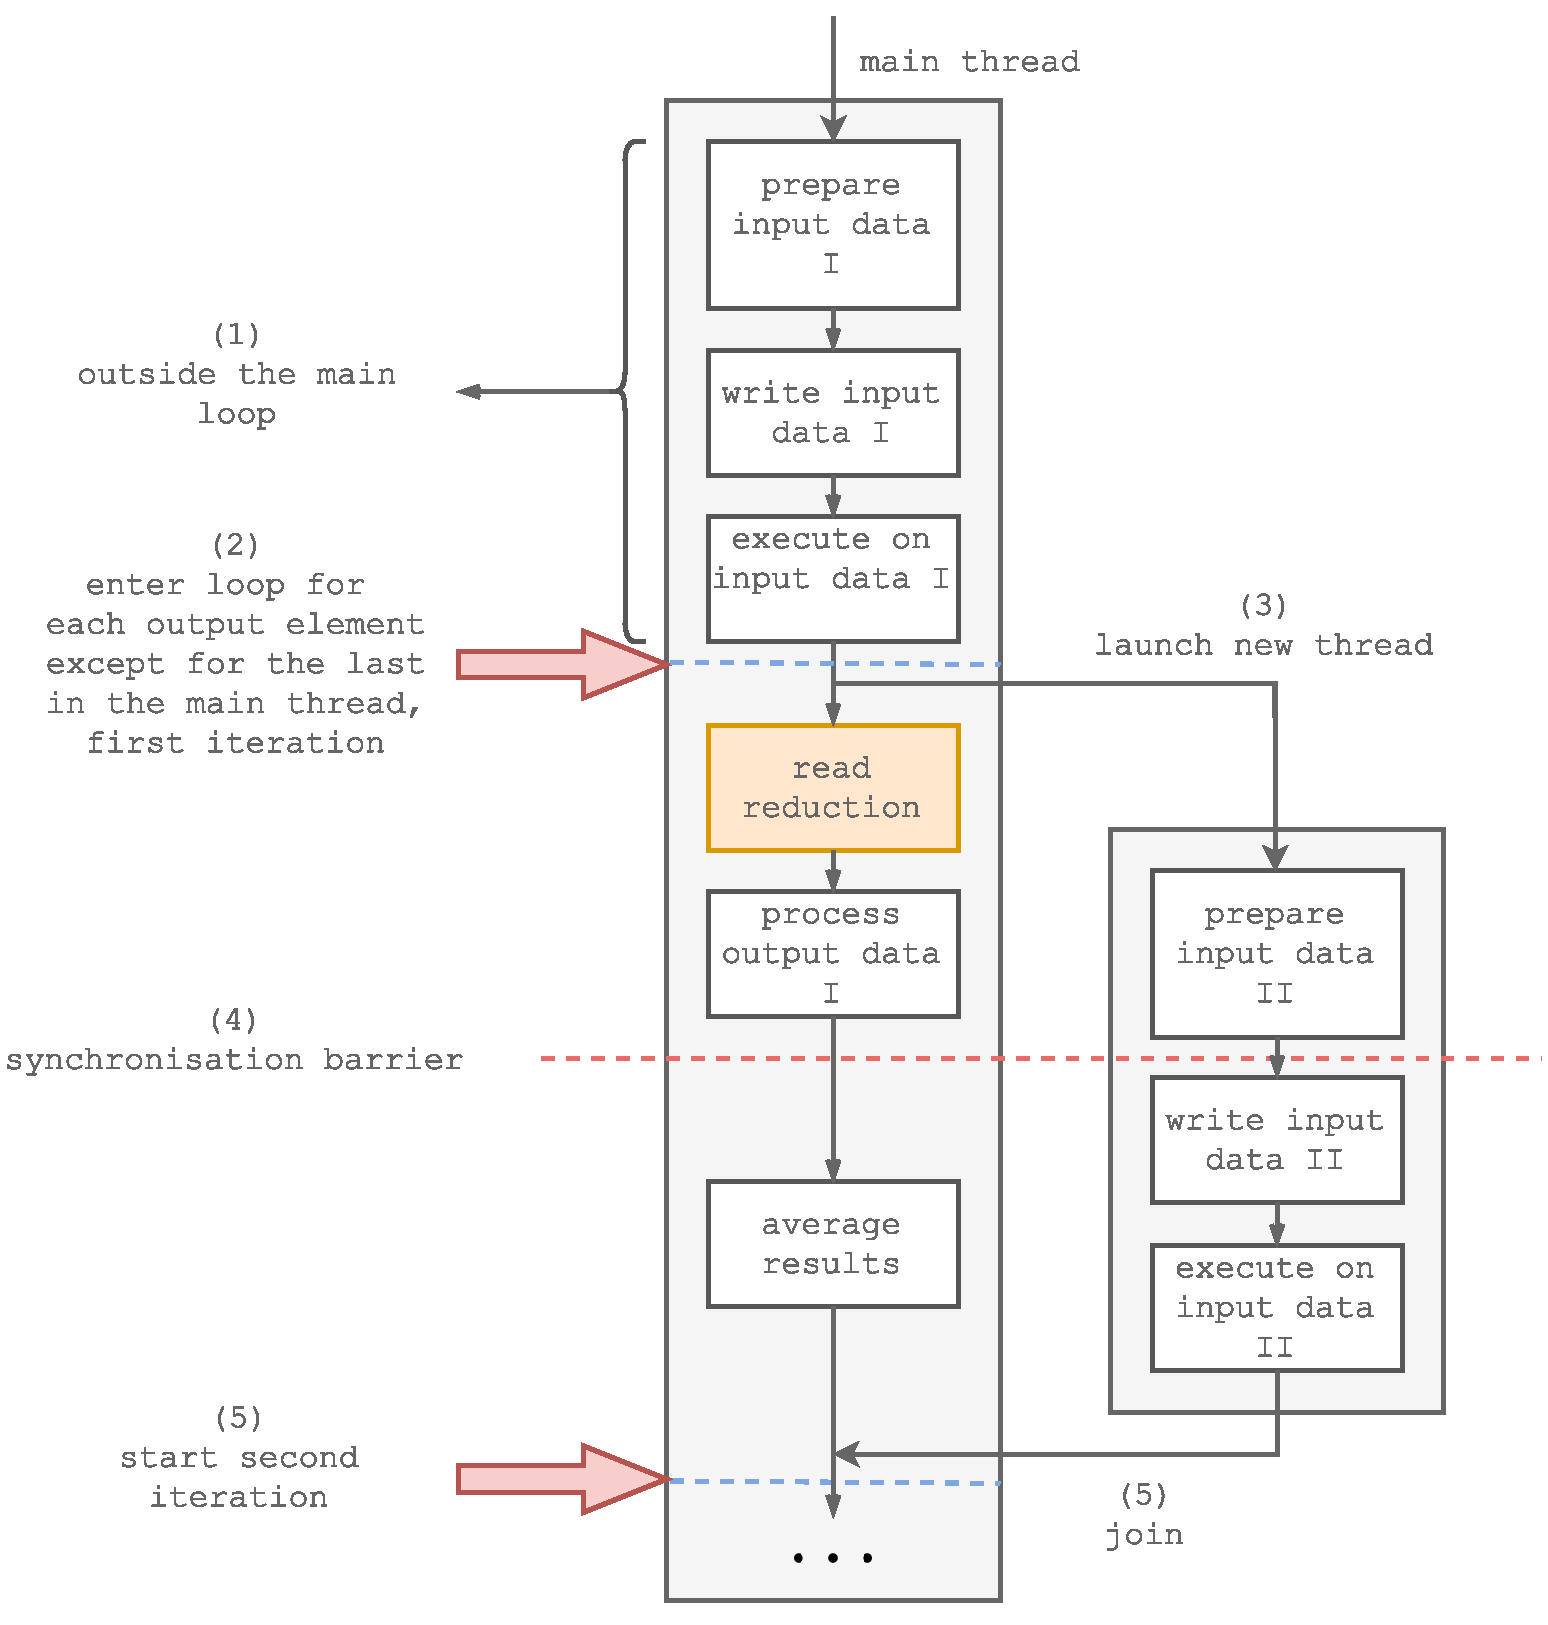
\includegraphics[width=0.8\textwidth]{src/img/autocorr-parallel}
    \caption{Modul de lucru distribuit al blocului de autocorelație}
    \label{fig:autocorr-parallel}
\end{figure}

Blocul de autocorelație are un număr de intrări egal cu numărul de antene al
sistemului și, pentru compararea timpului de execuție dintre blocul original și
cel care folosește kernelul de autocorelație, am aplicat pe fiecare intrare un
fișier cu o dimensiune de \SI{12}{MB}, deci cu un număr de 1,5 milioane de
eșantioane de numere complexe, având părțile reală și imaginară reprezentate în
virgulă mobilă, simplă precizie. În Figura \ref{fig:autocorr-time-2048} este
ilustrată o comparație între timpul de execuție obținut cu cele două blocuri
pentru o captură de 2048 de elemente și o suprapunere de 512 elemente, pentru
sisteme cu 4, 8, 16 și 32 antene. În medie, timpul de execuție este de 4 ori mai
mic decât cel inițial pentru cel puțin 8 antene, dar pentru anumite configurații
de antene care permit o mai bună folosire a resurselor, cum este cazul
sistemului de antene cu 16 elemente, timpul de execuție poate fi de până la 7
ori mai mic. \\

După cum a fost precizat în Secțiunea \ref{sec:kernel-autocorr}, dacă dorim să
folosim un șir de 64 de antene, putem avea o captură a autocorelației de maxim 1024
de eșantioane. Performanțele obținute de către blocul de autocorelație căruia
i-au fost aplicate la intrare fișiere de câte \SI{8}{MB} (1 milion de
eșantioane), care funcționează cu o dimensiune a capturii de 1024 de eșantioane
și o suprapunere de 256 de eșantioane pentru sisteme cu 4, 8, 16, 32 și 64
antene, sunt prezentate în Figura \ref{fig:autocorr-time-1024}. Folosind până la
8 antene, rezultatele sunt similare cu cele obținute în cazul anterior, dar
crescând acest număr, putem obține un timp de execuție de 6 - 7 ori mai mic
folosind 16 și 64 antene, sau chiar de aproape 10 ori mai mic pentru un sistem
cu 32 de antene. Aceste diferențe se datorează faptului că, fiind necesar un număr
mai mic de eșantioane ale semnalului de intrare (1024 față de 2048), ele vor fi
disponibile mai rapid și, în majoritatea cazurilor, \textit{scheduler}-ul GNU
Radio va apela funcția \code{work} cu un număr mai mare de date de ieșire pe
care le poate produce în acea execuție. Datorită faptului că blocul de
autocorelație care folosește kernelul ConnexArray pregătește datele de intrare
pentru următorul element de ieșire în paralel cu procesarea necesară producerii
elementului de ieșire curent, el va beneficia de pe urma apelării funcției
\code{work} cu un număr cât mai mare de elemente de ieșire, motiv pentru care
vom obține performanțe mai bune în cazul în care folosim o captură cu un număr
mai mic de eșantioane.

\begin{minipage}[h]{.5\textwidth}
  \centering

  \pgfplotstableread{assets/graph-data/autocorr-2048-original.dat}{\orig}
  \pgfplotstableread{assets/graph-data/autocorr-2048-kernel.dat}{\kernel}

  \begin{tikzpicture}[scale=0.9]
    \begin{axis}[
        ymin=0,
        ymax=100,
        xmin=0,
        xmax=35,
        xlabel=Antene,
        ylabel=Timp (s),
        every axis plot/.append style={thick},
        ylabel near ticks,
        legend pos=north west,
        xtick=data
      ]
      \addplot[mark=*,color=teal] table [x={antennas}, y={time}] {\orig};
      \addlegendentry{Implementare originală};

      \addplot[mark=square*,color=orange] table [x={antennas}, y={time}] {\kernel};
      \addlegendentry{Implementare accelerată};

    \end{axis}
  \end{tikzpicture}

  \captionsetup{justification=centering}
  \captionof{figure}{Timpul de execuție al blocului de autocorelație pe
  procesorul ARM pentru o captură de 2048 eșantioane}
  \label{fig:autocorr-time-2048}
\end{minipage}
~
\begin{minipage}[h]{.5\textwidth}
  \centering
  
  \vspace*{0.2cm}
  
  \pgfplotstableread{assets/graph-data/autocorr-1024-original.dat}{\orig}
  \pgfplotstableread{assets/graph-data/autocorr-1024-kernel.dat}{\kernel}

  \begin{tikzpicture}[scale=0.9]
    \begin{axis}[
        ymin=0,
        ymax=240,
        xmin=0,
        xmax=65,
        xlabel=Antene,
        ylabel=Timp (s),
        ylabel near ticks,
        every axis plot/.append style={thick},
        legend pos=north west,
        xtick=data
      ]
      \addplot[mark=*,color=lime!80!black] table [x={antennas}, y={time}] {\orig};
      \addlegendentry{Implementare originală};

      \addplot[mark=square*,color=violet] table [x={antennas}, y={time}] {\kernel};
      \addlegendentry{Implementare accelerată};

    \end{axis}
  \end{tikzpicture}

  \captionsetup{justification=centering}
  \captionof{figure}{Timpul de execuție al blocului de autocorelație pe
  procesorul ARM pentru o captură de 1024 eșantioane}
  \label{fig:autocorr-time-1024}
\end{minipage}

În privința preciziei, nu s-au observat modificări semnificative datorate
scăderii acestui număr de eșantioane, deoarece, prin simulări, s-a constatat că și
în acest caz se pot distinge surse de semnal distanțate la o diferență de
$1^{\circ}$ cu o acuratețe de $0.15^{\circ}$. \\

În ambele cazuri, performanțele cele mai scăzute se obțin pentru un număr de 4
antene, deoarece capacitatea memoriei aceeleratorului nu este complet
exploatată și nici nu evităm suficient de multe înmulțiri prin calcularea elementelor
de deasupra diagonalei principale, inclusiv.


%=============================================================================
% EVAL BLOC SPECTRU MUSIC
%=============================================================================
\section{Evaluarea performanțelor blocului ce calculează spectrul MUSIC}
\label{sec:eval-music}

\subsection{Utilizarea kernelului ce calculează produsul dintre un vector linie
și o matrice}
\label{sec:eval-music-vecmat}

Blocul GNU Radio care calculează spectrul MUSIC are o singură intrare, care
reprezintă autocorelația semnalului de intrare pe care, în funcție de numărul de
antene din sistem, o va interpreta ca pe o matrice liniarizată. În evaluarea
performanțelor, am aplicat pe această intrare date care provin dintr-un fișier
cu o dimensiune de \SI{8}{MB}, corespunzătoare a 1 milion de eșantioane de numere
fracționare pe 32 de biți. Atunci când sistemul va fi format dintr-un număr mai
mare de antene, datele vor fi ,,consumate'' în blocuri mai mici și execuția va
fi mai îndelungată. În Tabelul \ref{tab:prof-music-kernel-eval} sunt prezentate
cele mai importante rezultate obținute dintr-un profil al ciclilor de execuție
conform metodologiei din Secțiunea \ref{sec:met-eval-perf}, realizat pe acest
bloc izolat de lanțul MUSIC,  cu următoarea configurație: 
\begin{itemize}
  \item Număr antene: 4
  \item Număr semnale de intrare: 2
  \item Dimensiunea spectrului MUSIC: 1024
\end{itemize}

În acest caz, funcția care pregătește datele la ieșirea din accelerator este cea
mai problematică, deoarece se execută în buclă pentru fiecare bloc de date procesat, dar
proporția pe care o reprezintă din numărul total de cicli nu este
îngrijorătoare. În eventualitatea în care am crea un nou fir de execuție care să
se ocupe de această sarcină în paralel cu procesarea unui bloc următor de date,
ar trebui să ținem cont și de \textit{overhead}-ul introdus de acesta, care este
posibil să compenseze avantajul obținut prin paralelizare. Printre rezultate,
încă se găsesc funcții din biblioteca Armadillo, deoarece din înmulțirea
înlănțuită dintre un vector linie, o matrice și o coloană, doar primul produs se
realizează pe accelerator, rezultând un vector linie, care se înmulțeste apoi cu
ultimul vector coloană și explică apariția din tabel a simbolului
\code{cgemv\_}, corespunzător unei rutine BLAS pentru înmulțirea a doi vectori.\\

%=============================================================================
% Profiling table
%=============================================================================
\begin{table}[h]
\begin{center}
 \begin{tabular*}{\textwidth}{||c @{\extracolsep{\fill}} c @{\extracolsep{\fill}} c @{\extracolsep{\fill}}||}
% {||c c c||} 
 \hline
 Overhead  & Command & Symbol \\ [0.5ex] 
 \hline\hline
 9,45\% 
 &
 MUSIC\_lin\_array
 &
 \makecell{gr::doa::MUSIC\_lin\_array\_cnx\_impl:: \\
 prepareOutDataConnex}
 \\ 
 
 \hline
 7,58\%
 &
 MUSIC\_lin\_array
 &
 \makecell{arma::Mat<std::complex<float> >::init\_warm}
 \\
 
 \hline
 7,13\%  
 &
 MUSIC\_lin\_array
 &
 \makecell{cgemv_}
 \\
 
 \hline
 5,75\%  
 &
 MUSIC\_lin\_array
 &
 \makecell{arma::subview<std::complex<float> >::extract}
 \\
 
 \hline
 5,05\%  
 &
 MUSIC\_lin\_array
 &
 \makecell{\_\_copy\_from\_user}
  
 \\ [1ex] 
 \hline
\end{tabular*}
\end{center}
\caption{Profil pentru blocul care calculează spectrul MUSIC cu un kernel ConnexArray}\label{tab:prof-music-kernel-eval}
\end{table}


Constatăm, deci, că singurele îmbunătățiri cu un impact mai mare care ar putea
fi efectuate sunt legate de folosirea la capacitate maximă a memoriei
acceleratorului. Reamintim că aceasta depinde atât de numărul de antene din
sistem, cât și de dimensiunea spectrului MUSIC, cea din urmă având impact asupra
acurateței măsurătorii. Cu cât se efectuează mai puține înmulțiri într-o
execuție a kernelului, cu atât întârzierea introdusă de transferul I/O va deveni
mai semnificativă. \\

\begin{minipage}[h]{1\textwidth}
  \centering
  \pgfplotstableread{assets/graph-data/music-1024-orig.dat}{\orig}
  \pgfplotstableread{assets/graph-data/music-1024-kernel.dat}{\kernel}

  \begin{tikzpicture}[scale=0.9]
    \begin{axis}[
        ymin=0,
        ymax=200,
        xlabel=Antene,
        ylabel=Timp (s),
        ylabel near ticks,
        every axis plot/.append style={thick},
        legend pos=north east,
        xtick=data
      ]
      \addplot[mark=*,color=lime!80!black] table [x={antennas}, y={time}] {\orig};
      \addlegendentry{Implementare originală};

      \addplot[mark=square*,color=violet] table [x={antennas}, y={time}] {\kernel};
      \addlegendentry{Implementare accelerată};

    \end{axis}
  \end{tikzpicture}

  \captionsetup{justification=centering}
  \captionof{figure}{Timpul de execuție al blocului ce calculează spectrul MUSIC
  cu 1024 elemente}
  \label{fig:music-time-1024}
\end{minipage}


Pentru configurația acceleratorului ConnexArray folosită și aranjarea
elementelor propusă în Secțiunea \ref{sec:kernel-mult-array}, pentru 4 antene și
o dimensiune a spectrului MUSIC de 1024 de elemente, de exemplu, ar fi ocupate doar
256 de linii din LS, deci un sfert din capacitatea sa totală. Atunci când vom
calcula numărul de linii din LS disponibile pentru stocarea vectorilor de
intrare, dacă avem nu număr mai mic sau egal de 32 de antene, putem să transferăm
elementele matricei de intrare în registre înaintea stocării vectorilor, pentru
ca aceasta să fie în întregime disponibilă pentru ei. Pentru mai mult de 32 de
antene, nu dispunem de suficiente registre pentru a realiza acest lucru, deci
vom folosi varianta inițială. \\

În acest caz, pentru o dimensiune a spectrului MUSIC de 1024 elemente și pentru
configurații de sisteme cu 4, 8, 16, 32 și 64 antene, timpii de execuție
obținuți sunt redați în Figura~\ref{fig:music-time-1024}. Ca și în cazul
kernelului pentru autocorelație, pentru un număr mic de antene (de exemplu, 4
sau 8) performanțele sunt similare cu ale blocului inițial care nu folosește
acceleratorul. Crescând numărul de antene, însă, este utilizată mai eficient
capacitatea de stocare a acceleratorului și timpul de execuție se înjumătățește
față de cel al blocului inițial.

\subsection{Utilizarea kernelului ce calculează produsul înlănțuit dintre un
vector linie, o matrice și un vector coloană}
\label{sec:eval-music-chained}

În privința kernelului care calculează produsul dintre un vector linie, o
matrice și un vector coloană, s-a observat că singura situație în care oferă
rezultate mai bune este pentru un număr mic de antene (de exemplu, 4), deoarece
pentru dimensiuni mai mari ale șirurilor de antene și, implicit, ale dimensiunii
vectorilor, memoria locală a acceleratorului este folosită ineficient, trebuind
să ocupăm mai multe linii de stocare pentru a efectua o singură înmulțire. Acest
lucru conduce la procesarea în blocuri mai mici și timpul necesar transmiterii
datelor pe interfața AXI către accelerator nu mai este neglijabil. \\

Figura \ref{fig:music-time-versions} prezintă o comparație între timpii de
execuție obținuți cu blocul ce calculează spectrul MUSIC folosind un kernel
pentru produsul înlănțuit, în aceleași condiții descrise în
Secțiunea~\ref{sec:eval-music-vecmat}, și cei prezentați și în
Figura~\ref{fig:music-time-1024} pentru același bloc în varianta originală și în
varianta ce conține kernelul pentru înmulțirea dintre un vector și o matrice.

\begin{minipage}[h]{1\textwidth}
  \centering
  \pgfplotstableread{assets/graph-data/orig-music.dat}{\orig}
  \pgfplotstableread{assets/graph-data/simple-music.dat}{\simple}
  \pgfplotstableread{assets/graph-data/chained-music.dat}{\chained}

  \begin{tikzpicture}[scale=1]
    \begin{axis}[
        xmode=log,
        ybar, axis on top,
        height=8cm, width=15.5cm,
        bar width=0.8cm,
        ymajorgrids, tick align=inside,
        major grid style={draw=white},
        enlarge y limits={value=.1,upper},
        ymin=0, ymax=170,
        axis x line*=bottom,
        axis y line*=left,
        y axis line style={opacity=0},
        tickwidth=0pt,
        enlarge x limits=true,
        legend style={
            at={(0.5,-0.2)},
            anchor=north,
            legend columns=-1,
            /tikz/every even column/.append style={column sep=0.2cm}
        },
        ylabel=Timp (s),
        xlabel=Antene,
        xticklabels={4, 8, 16, 32, 64},
        xtick=data,
        nodes near coords={
        \pgfmathprintnumber[precision=1]{\pgfplotspointmeta}
       },
       every node near coord/.append style={font=\small}
    ]      
    
      \addplot [draw=none,fill=orange!60!white] table [x={antennas}, y={time}] {\orig};

      \addplot [draw=none,fill=violet!60!white] table [x={antennas}, y={time}] {\simple};

      \addplot [draw=none,fill=teal!60!white] table [x={antennas}, y={time}] {\chained};
      \legend{Original, Kernel vector x matrice, Kernel vector x matrice x
      vector}
    \end{axis}
  \end{tikzpicture}

  \captionsetup{justification=centering}
  \captionof{figure}{Timpul de execuție al lanțului de procesare MUSIC în
  cele trei variante pentru o
  dimensiune a spectrului MUSIC de 1024 de elemente}
  \label{fig:music-time-versions}
\end{minipage}


\subsection{Concluzii}
Având în vedere rezultatele obținute, putem considera justificabilă doar
folosirea kernelului ce înmulțește un vector linie cu o matrice pătratică în
calculul spectrului MUSIC, motiv pentru care, pentru simplitate, ne vom referi
în continuare la acesta sub numele de ,,kernel MUSIC''. Kernelul care efectuează
înmulțirea dintre un vector linie, o matrice pătratică și un vector coloană se
pretează doar pentru tablouri de dimensiuni mici, până în 4 elemente. Deoarece
configurațiile sistemelor radio sunt, cel mai adesea, statice, în sensul că un
echipament nu își va schimba în mod dinamic numărul de antene, alegerea unei
anumite variante se va face fără niciun fel de \textit{overhead}.

%=============================================================================
% EVAL LANT MUSIC
%=============================================================================
\section{Evaluarea performanțelor lanțului de procesare MUSIC folosind ConnexArray}
\label{sec:eval-music-chain}

În momentul de față, kernelurile create nu se pot folosi simultan în lanțul de
procesare MUSIC, deoarece nu există implementată, momentan, o modalitate de
gestionare a accesului la resurse pentru procesări diferite pe accelerator.
Acest lucru ar presupune asigurarea faptului că execuția unui kernel se face pe
un set de date dorit, că un bloc nu citește elementele din coada de
reducție destinate altui bloc și, în plus, o metodă de selectare a blocului care
primește acces la accelerator. Pentru a stabili dacă un astfel de mecanism este
eficient, trebuie efectuată o analiză a gradului de utilizare a acceleratorului
relativ la cel al blocului. Dacă se constată că acesta este sub-utilizat, atunci
acceleratorul ar putea fi folosit succesiv de mai multe blocuri fără
întârzieri prea mari. \\

O alternativă la implementarea unui astfel de mecanism, în cazul în care se
constată că un accelerator nu poate suporta execuțiile mai multor blocuri de
procesare, poate fi existența a cel puțin un acceleratoar în plus în FPGA,
astfel încât fiecare bloc să aibă suportul său hardware dedicat, cu costul
creșterii complexității sistemului și al consumului de putere. \\

Întrucât niciuna dintre aceste situații nu este, momentan, posibilă, ne vom
rezuma la analiza fiecărui kernel integrat separat în lanțul de procesare MUSIC,
căruia i-au fost aplicate la intrare patru seturi de date citite din fișiere,
fiecare de o dimensiune de \SI{8}{MB}: două pentru semnale de intrare
cosinusoidale cu frecvențe de \SI{10}{kHz} și \SI{20}{kHz} și două pentru
sursele de zgomot gaussian, iar întregul lanț de procesare a primit următorii
parametri:
\begin{itemize}
  \item Frecvența de eșantionare: \SI{320}{kHz}
  \item Numărul de semnale de intrare: 2
  \item Numărul de antene: 4, 8, 16, 32 sau 64
  \item Dimensiunea spectrului MUSIC: 1024 elemente
  \item Dimensiunea capturii autocorelației: 1024 pentru cazul cu 64 de antene
  și 2048 eșantioane, în rest\footnote{În cazul sistemelor cu 64 antene,
  schimbăm dimensiunea capturii autocorelației, deoarece aceasta poate fi maxim
  1024 utilizând kernelul pentru autocorelație în care date nu se împart în mai
  multe blocuri de procesare.}
  \item Suprapunerea dintre capturi: 256 pentru cazul cu 64 de antene și 512
  eșantioane, în rest
\end{itemize}

\begin{minipage}[h]{1\textwidth}
  \centering
  \pgfplotstableread{assets/graph-data/chain-1024-orig.dat}{\orig}
  \pgfplotstableread{assets/graph-data/chain-1024-music.dat}{\music}
  \pgfplotstableread{assets/graph-data/chain-1024-autocorr.dat}{\autocorr}

  \begin{tikzpicture}[scale=1]
    \begin{axis}[
        xmode=log,
        ybar, axis on top,
        height=8cm, width=15.5cm,
        bar width=0.8cm,
        ymajorgrids, tick align=inside,
        major grid style={draw=white},
        enlarge y limits={value=.1,upper},
        ymin=0, ymax=370,
        axis x line*=bottom,
        axis y line*=right,
        ylabel near ticks, 
        yticklabel pos=right,
        y axis line style={opacity=0},
        tickwidth=0pt,
        enlarge x limits=true,
        legend style={
            at={(0.5,-0.2)},
            anchor=north,
            legend columns=-1,
            /tikz/every even column/.append style={column sep=0.4cm}
        },
        ylabel=Timp (s),
        xlabel=Antene,
        xticklabels={4, 8, 16, 32, 64},
        xtick=data,
        nodes near coords={
        \pgfmathprintnumber[precision=1]{\pgfplotspointmeta}
       },
       every node near coord/.append style={font=\small}
    ]      
    
      \addplot [draw=none,fill=orange!60!white] table [x={antennas}, y={time}] {\orig};

      \addplot [draw=none,fill=teal!60!white] table [x={antennas}, y={time}] {\music};

      \addplot [draw=none,fill=violet!60!white] table [x={antennas}, y={time}] {\autocorr};
      \legend{Original, Kernel MUSIC, Kernel autocorelație}
    \end{axis}
  \end{tikzpicture}

  \captionsetup{justification=centering}
  \captionof{figure}{Timpul de execuție al lanțului de procesare MUSIC pentru o
  dimensiune a spectrului MUSIC de 1024 de elemente}
  \label{fig:music-chain-1024}
\end{minipage}


Rezultatele obținute pentru timpii de execuție sunt sintetizate în Figura
\ref{fig:music-chain-1024}. Am observat că, per ansamblu, nu există îmbunătățiri
semnificative în timpul de execuție al întregului lanț de procesare dacă
integrăm, pe rând, câte unul dintre blocurile optimizate, deși evaluate
individual fiecare dintre ele a prezentat un timp de execuție mult mai mic decât
varianta originală. O îmbunătățire constantă s-a evidențiat doar în privința
variantei care folosește kernelul pentru autocorelație, care pentru 16 și 32 de
antene a obținut un timp de execuție cu 35\% mai redus, iar pentru un număr de
64 de antene ambele variante care folosesc acceleratorul au avut un timp de
execuție de aproximativ 5 minute, față de cele 6 minute ale implementării
originale. \\

Motivul pentru care performanțele în întreg ansamblul nu le ating pe cele
constatate pentru fiecare bloc în parte provine din faptul că, după s-a putut vedea în
Capitolul \ref{chapter:impl}, în Tabelul \ref{tab:prof-zedboard}, ponderea
blocurilor de autocorelație și a celui care calculează spectrul MUSIC în numărul
total de cicli de execuție pe procesor a fost similară, de 18,97\% și,
respectiv, 13,68\%, iar blocurile depind unul de celălalt în privința schimbului
de date. Optimizându-l doar pe unul dintre ele, celălalt bloc va reprezenta un
\textit{bottleneck}, blocând fluxul de date, și timpul de execuție va fi, per
total, similar cu cel al variantei originale, lucru observat și cu ajutorul
utilitarului \textbf{top} disponibil pe sistemul de operare Linux, vizualizând
statistici pentru fiecare fir de execuție. \\


În Tabelele \ref{tab:prof-chain-autocorr-k} și \ref{tab:prof-chain-music-k} sunt
prezentate principalele rezultate ale unor profile ale ciclilor de execuție
efectuate pe întregul lanț de procesare, în situația în care folosim kernelul
pentru autocorelația unui semnal și, respectiv, kernelul care calculează
spectrul MUSIC.  În Tabelul~\ref{tab:prof-chain-autocorr-k}  observăm că, atunci
când folosim kernelul de autocorelație, sarcina principală de procesare, de până
la 43,51\% din ciclii totali de execuție, cade în aria blocului care calculează
spectrul MUSIC și, invers, când folosim kernelul MUSIC în întregul lanț de
procesare, punctul critic ajunge în blocul de autocorelație, care realizează
42,08\% din procesare, după cum se observă în
Tabelul~\ref{tab:prof-chain-music-k}, ceea ce dovedește, încă o dată,
interdependența dintre cele două blocuri și dificultatea de a le analiza
separat.

\begin{table}
\parbox{.5\textwidth}{
\centering
\resizebox{0.5\textwidth}{!}{
\begin{tabular}
{||c  c  c ||}

\hline
 Overhead  & Command & Symbol \\ [0.5ex] 
\hline\hline

\hline
43,51\%
&
MUSIC\_lin\_array
&
cgemm\_
\\

\hline
12,16\%
&
autocorrelate_cnx
&
prepareInData
\\

\hline
2,94\%
&
autocorrelate\_cnx
&
\makecell{std::complex \\ <float>::imag}
\\

\hline
\end{tabular}
}
\centering
\caption{Profil de execuție pentru lanțul MUSIC folosind kernelul de
autocorelație}
\label{tab:prof-chain-autocorr-k}
}
%\hfill
\parbox{.5\textwidth}{
\centering
\resizebox{0.5\textwidth}{!}{
\begin{tabular}
{||c  c  c ||}

\hline
 Overhead  & Command & Symbol \\ [0.5ex] 
\hline\hline

\hline
42,08\%
&
autocorrelate
&
cgemm\_
\\

\hline
3,69\%
&
autocorrelate
&
arma::eopcore[...]
\\

\hline
3,40\%
&
multiply\_matrix
&
\makecell{\_\_mulsc3 \\
\\}
\\


\hline
\end{tabular}
}
\centering
\caption{Profil de execuție pentru lanțul MUSIC ce folosește kernelul MUSIC}
\label{tab:prof-chain-music-k}
}
\end{table}


% \todo{Obțin date din blocurile gnuradio despre starea bufferelor ca sa pot sa
% extrag ceva date despre cum se blocheaza} \\


%=============================================================================
% PROFIL PUTERE
%=============================================================================
%\section{Profil al consumului de putere}
%\label{sec:eval-power}
%
%\todo{TODO?}


%=============================================================================
% CONCLUZII
%=============================================================================
\section{Concluzii referitoare la performanțele obținute}
\label{sec:eval-concl}

În concluzie, performanțele blocurilor considerate individual, constând în timpi de
execuție de 4 - 7 ori mai mici, în cazul blocului care folosește kernelul
pentru autocorelație, și de 2 ori mai mici, în cazul blocului care folosește
kernelul pentru calculul spectrului MUSIC, le fac demne de luat în considerare
în implementarea algoritmului MUSIC și, în cazul în care ar putea fi folosite
simultan, ar conduce, cu siguranță, și la îmbunătățiri în timpul de execuție al
întregului ansamblu, după cum reiese din profilurile de execuție realizate
pentru acesta. \\

O altă îmbunătățire posibilă ar fi existența unui sport hardware pentru
conversia datelor din virgulă mobilă în virgulă fixă, operație care poate deveni
deosebit de costisitoare, după cum s-a observat în profilurile realizate în
Secțiunile \ref{sec:eval-autocorr} și \ref{sec:eval-music}. \\

S-au observat îmbunătățiri mai accentuate pentru configurații cu mai mult de 16
antene, rezultat relevant, de exemplu, în contextul sistemelor de
telecomunicații actuale care folosesc tehnici MIMO sau Massive MIMO cu un număr
mare de antene și care pot beneficia de pe urma algoritmilor DoA pentru a obține
informații despre sursa unui semnal și pentru a facilita \textit{beamforming}-ul
3D~\cite{wang2015two}. \\

Având în vedere consumul de putere redus al platformei folosite, se poate lua în
considerare folosirea sa în componența unor micro-stații de bază, a căror
principală limitare este consumul de putere, sau, dacă resursele de putere sunt
mai mari, putem imagina un sistem care să cuprindă o serie de mai multe
acceleratoare ConnexArray controlate de către un procesor mai puternic. În
rețele celulare eterogene, de exemplu, macro-celulele lucrează alături de micro,
pico sau femto celule care au o putere de transmisiune foarte mică și pot fi
folosite în mod dinamic în funcție de traficul existent în rețea, pentru a
obține o modelare cât mai eficientă a consumului de
putere~\cite{lorincz2012measurements}. \\

Posibilitățile de folosire a kernelurilor propuse în algoritmi de localizare a
sursei unui semnal nu sunt restrânse doar la algoritmul MUSIC, întrucât și alți
algoritmi de localizare (de exemplu, ESPRIT) folosesc autocorelația în procesul
de estimare a unghiului de incidență. În plus, generalitatea produselor dintre
vectori și matrice le poate face potrivite și pentru alte tipuri de aplicații în
procesarea digitală de semnale, iar faptul că kernelurile au fost integrate în
blocuri GNU Radio de sine stătătoare facilitează integrarea lor în acestea.

